% #############################################################################
% This is Chapter 1
% !TEX root = ../main.tex
% #############################################################################
% Change the Name of the Chapter i the following line
\fancychapter{Introduction}
\cleardoublepage
% The following line allows to ref this chapter
\label{chap:intro}
At the start of the millennium, Coats et. al ~\cite{Coats2000} predicted that streaming would become the future of audio media consumption. With respect to music streaming services and corresponding developments around related technologies and the internet, early studies anticipated the stagnation and ultimate demise of traditional media, such as terrestrial radio ~\cite{Ala-Fossi2008}. More recent research, however, appears to contradict these predictions, revealing the sustained popularity of traditional radio broadcasting. ~\cite{DangNguyen2012, Waits2007}. Indeed, in large parts of the world, traditional radio remains strong and continues to co-exist alongside newer streaming services, albeit with the important caveat that younger audiences are diminishing ~\cite{Albarran2007}. 
%Many audio listeners state that these traditional mediums haven't followed the technological evolution that is now undergoing. This has given some advantage to music streaming services, which are becoming the preferred way for users to experience and enjoy audio content.

Streaming has rapidly become the standard delivery method for digital entertainment content ~\cite{Swaminathan2013}, with the music industry forming an integral part of this interactive mode of media conveyance. In recent years, platforms such as Spotify, Apple Music, and Tidal have emerged as  some of the more predominant and thriving services for on-demand media consumption, offering users new and easier ways to access, listen to, and discover songs, artists ~\cite{Weijters2014} and, more recently, podcasts to match their tastes. Specifically, audio streaming services enable listeners to access and discover an almost limitless selection of content ~\cite{Morris2015}. With their ubiquity and large catalogues of recorded music and podcasts, along with social functions - such as the ability to create and collaborate on playlists, group listening, and shared activity notifications - audio streaming services offer listeners an enticing array of experiences, resulting in the widespread adoption of these services. ~\cite{Mantymaki2015}

Traditional radio, on the other hand, delivers a connection to the outside world through the disclosure of important information in a succinct way. More importantly, and in contrast to music streaming services, it is difficult for radio stations to make their song selection appealing to every listener, which in return makes them get worn-out and tired of tuning in to radio stations. 

Yet, traditional terrestrial radio's popularity has remained very strong in recent years. ~\cite{Albarran2007} This is, in part, due to the human connection this medium provides, and which other modern solutions are taking away ~\cite{Waits2007}. The 'social presence element', described by Short et. al ~\cite{JohnShortEderynWilliams1976} as "the degree to which a particular medium allows communicators to feel other people as being present psychologically", is lacking in music streaming services. The authors state that, in conjunction with the lack of nonverbal cues —  which makes the communication quite limited — there is a direct and indirect impact on users’ behavioral intention or actual use of technological platforms, such as music streaming services ~\cite{Wang2014}.

From the beginning of its adoption, terrestrial radio's strengths were ubiquity of access, ease of use, and the local nature of its content, as stated by the North American Broadcasters Association (NABA) ~\footnote{\href{https://nabanet.com/wp-content/uploads/2019/03/NGR-WG-Value-Proposition-of-Radio-in-a-Connected-World-2019-03-15.pdf}{The Value Proposition Of Radio In A Connected World — NABA Next Generation Radio Working Group, 2019}}. Furthermore, according do Priestman et. al ~\cite{Priestman2005}, one of the most compelling reasons for people to listen to it is because of the intimacy of audio - a person listening to radio is alone with the announcer or artist, even if other people are physically present, and much of the fascination of audio is the imagination it requires on the part of the listener to actively visualize. Waits et. al ~\cite{Waits2007} also states that listening to the radio, though experienced individually, is often a communal act, which sets our relationship to traditional radio to be determined by a certain expectation that it will be authentic and sociable.

Bringing all together, we can conclude that there is a lack of solutions that aim to improve the audio media consumers' experience. Music streaming services are convenient and highly popular because they allow listeners to not only enjoy their favorite songs on demand, but also to discover brand new artists that match their music taste. On the downside, they eliminate the human connection that traditional terrestrial radio stations provide, as there isn't someone on the other side of the line interacting with the listener, nor communicating information such as news, weather, or traffic information. Therefore, listeners loose their connection to the outside world while pivoting themselves on music streaming services. To try to improve this experience, we have started by asking ourselves: how can audio media consumers' music streaming and traditional terrestrial radio habits be best represented in an integrated and personalized experience that may be shared within small networks of friends and family?

In this work, we explore how we can create a solution, named 'Sterio', that aims to merge the best features of both these audio listening mediums — music streaming services and traditional terrestrial radio  — in a platform that is user-focused from its inception. In a first stage, we conduct research on the currently available services. Then, we apply three user research techniques, so that we are able to have a better understanding on the users' audio media consuming habits. Finally, and most importantly, we apply the speed dating methodology, which will guide us on the development of a solution that aims to improve users' experience. We exploit all the user-centered design principles we have employed, so that the final solution suits the user, rather than forcing the user to suit our solution. In the end, a general purpose platform that creates a personalized, integrated and social experience for its users will emerge. 
% #############################################################################
\section{Goals}
Pellentesque nibh felis, eleifend id, commodo in, interdum vitae, leo. 
 Praesent mauris \ac{SD} and \ac{HD} volutpat ligula eget enim \acp{WLAN} and 3G\slash 4G \acp{WWAN}.\todo[color=cyan!40, author=RC]{use of ACRONYMS that are defined in file ``Chapters/Thesis-MSc-Aconyms.tex''}

Praesent eu elit. Ut eu ligula. Class aptent taciti sociosqu ad litora torquent per conubia nostra, per inceptos hymenaeos. Maecenas elementum augue nec nisl. Proin auctor lorem at nibh. Curabitur nulla purus, feugiat id, elementum in, lobortis quis, pede. Vivamus sodales adipiscing sapien. Vestibulum posuere nulla eget wisi. Integer volutpat ligula eget enim. Suspendisse vitae arcu. Quisque pellentesque. Nullam consequat, sem vitae rhoncus tristique, mauris nulla fermentum est, bibendum ullamcorper sapien magna et quam. Sed dapibus vehicula odio. Proin bibendum gravida nisl. Fusce lorem. Phasellus sagittis, nulla in hendrerit laoreet, libero lacus feugiat urna, eget hendrerit pede magna vitae lorem. 
 
Aliquam erat \ac{WLAN} volutpat \ac{CPU} mauris nulla fermentum est \ac{OS} Fusce magna mi, porttitor quis, convallis eget, sodales ac, urna.
Pellentesque nibh felis, eleifend id, commodo in, interdum vitae, leo. Praesent eu elit. Ut eu ligula. Class aptent taciti sociosqu ad litora torquent per conubia nostra, per inceptos hymenaeos. Maecenas elementum augue nec nisl. Please notice the use of automatic referencig to objects such as Figures, Tables, equations, Algorithms, sections of a document, etc. by using the command \verb:\Cref{ref}: as in this case pointing to \Cref{fig:cashed}.\todo[color=cyan!40, author=RC, fancyline]{the correct Name of the float object, in this case a Figure, is determined by the system}

\begin{figure}[h]
\centering
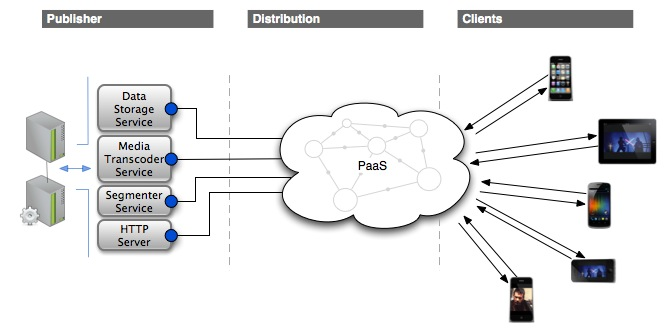
\includegraphics[width=0.9\textwidth]{./Images/cashed5}
\caption{Ecosystem}
\label{fig:cashed}
\end{figure}

Proin auctor lorem at nibh. Curabitur nulla purus, feugiat id, elementum in, lobortis quis, pede. Vivamus sodales adipiscing sapien. Vestibulum posuere nulla eget wisi. Integer volutpat ligula eget enim. Suspendisse vitae arcu. Quisque pellentesque. Nullam consequat, sem vitae rhoncus tristique, mauris nulla fermentum est, bibendum ullamcorper sapien magna et quam. Sed dapibus vehicula odio. Proin bibendum gravida nisl. Fusce lorem. Phasellus sagittis, nulla in hendrerit laoreet, libero lacus feugiat urna, eget hendrerit pede magna vitae lorem. Praesent mauris Class aptent taciti sociosqu ad litora torquent per conubia nostra, per inceptos hymenaeos H.264\slash \ac{AVC} standard, sem vitae rhoncus tristique \ac{SVC} \cite{Fraunhofer-Heinrich-Hertz-Institute:2013fk,ISO:H-264} nulla in hendrerit laoreet, libero lacus feugiat urna, eget hendrerit pede magna vitae lorem.

\textcolor{violet}{You can use in-paragraph lists with this construct for: 
\begin{inparaenum}[(a)]
\item first case;
\item second case; and
\item third case,
\end{inparaenum}
making the text organized and fluid.}

Vivamus auctor leo vel dui. Aliquam erat volutpat. Phasellus nibh. Vestibulum ante ipsum primis in faucibus orci luctus et ultrices posuere cubilia Curae; Cras tempor. Morbi egestas, urna non consequat tempus, nunc arcu mollis enim, eu aliquam erat nulla non nibh. Duis consectetuer malesuada velit. Nam ante nulla, interdum vel, tristique ac, condimentum non, tellus. Proin ornare feugiat nisl. Suspendisse dolor nisl, ultrices at, eleifend vel, consequat at, dolor, morbi egestas, urna non consequat tempus, nunc arcu mollis enim, eu aliquam erat nulla non nibh.



Maecenas elementum augue nec nisl. Proin auctor lorem at nibh. Curabitur nulla purus, feugiat id, elementum in, lobortis quis, pede. Vivamus sodales adipiscing sapien. Vestibulum posuere nulla eget wisi. Integer volutpat ligula eget enim. Suspendisse vitae arcu. Quisque pellentesque.
% #############################################################################
\section{Document Structure}
This thesis is is organized as follows: \Cref{chap:intro} \todo[color=cyan!40, author=RC, fancyline]{references to doc sections/chapters are automatic}{}interdum vel, tristique ac, condimentum non, tellus. 
In \cref{chap:back} curabitur nulla purus, feugiat id, elementum in, lobortis quis, pede.
In \cref{chap:architecture} consequat ligula nec tortor. Integer eget sem. Ut vitae enim eu est vehicula gravida.
\Cref{chap:implement} morbi egestas, urna non consequat tempus, nunc arcu mollis enim, eu aliquam erat nulla non nibh in \cref{chap:evaluation}.
\Cref{chap:conclusion} suspendisse dolor nisl, ultrices at, eleifend vel, consequat at, dolor.